\section{Implementation}
  This meant that it was going to be ideal associating electronic hardware with
  each component of the kart. This was especially important as to minimise the
  delay for PID control of the actuators meant that a higher baud rate was
  required. 

  \subsection{Schematics}
  Using Altium Designer the schematics were laid out. Two techniques were used
  to minimise mistakes in the PCB design. One was to divide all the schematic
  sections onto separate sheets. The other was to be methodical and make notes
  on the sheets if something was not complete. Part of being methodical also
  meant making sure all components were well labelled, even some with comments
  next to them to help explain their existence. This meant when the schematics
  were printed off and reviewed by the whole team, mistakes could be easily
  spotted.
  
  \begin{figure}[h]
      \centering
      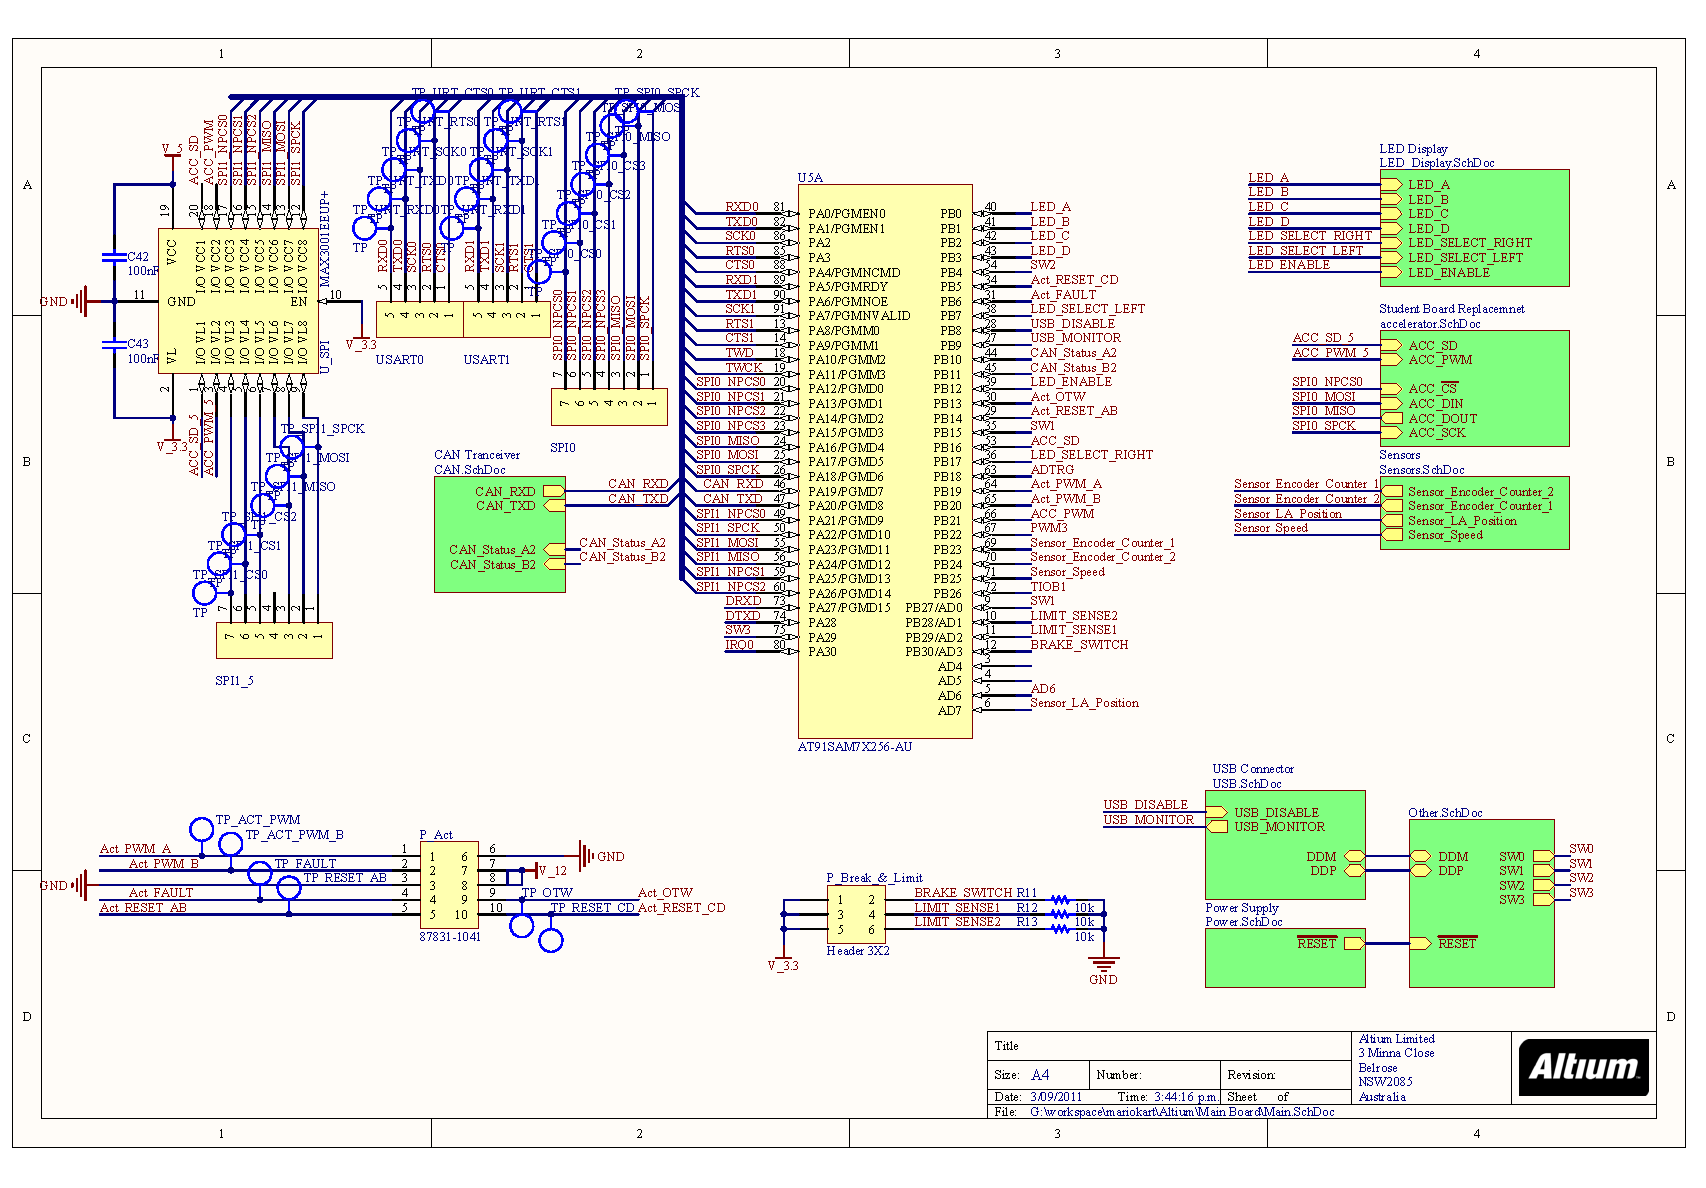
\includegraphics[width=\linewidth]{../../Presentation/Henry/Images/Schematic.pdf}
      \caption{Top level schematic for the main PCB.}
      \label{main-schematic}
  \end{figure}

  Figure \ref{main-schematic} shows the top level schematic with the MCU in the
  middle of the page. The green boxes on the sheet show where other sub sheets
  have been included and wired up. For example, doing this all the decoupling
  capacitors for the micro controller can be essentially hidden in one of these
  sub sheets. 

  \subsection{Components}

    \subsubsection{Motor Driver}
    The motor driver that was used is the DRV8432 made by Texas
    Instruments\cite{ti-motor-driver}. It is a dual full bridge PWM motor
    driver.  It has a split logic and driving voltage, so it is driven directly
    from the batteries, but the control logic is at 3.3V. It has a peak voltage
    of 50V and a maximum current of 12A which is more than we need for either
    of the actuators. Figure \ref{motorPCB} shows one of the two motor driver
    boards with a heat sink covering the motor driver IC.

     \begin{figure}[h]
         \centering
         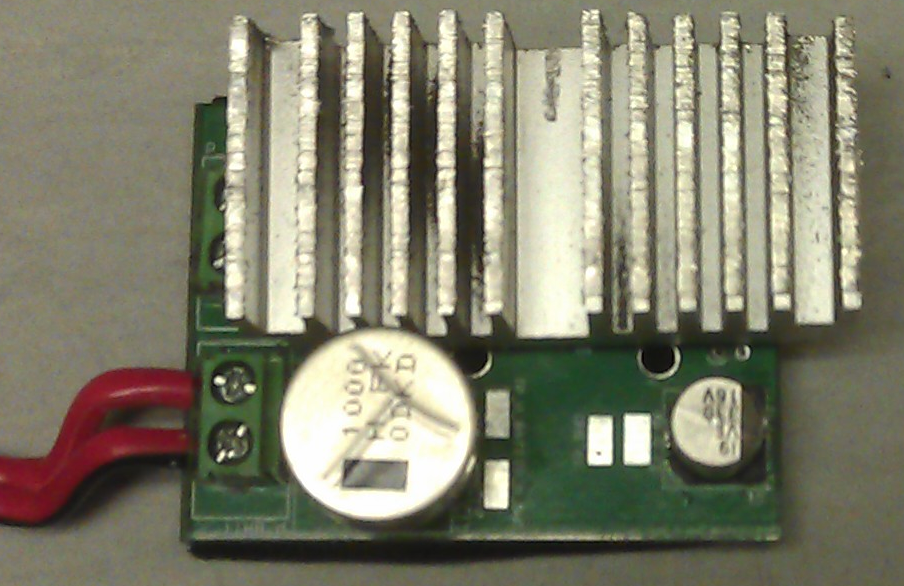
\includegraphics[width=.9\linewidth]{Images/motorPCB.png}
         \caption{Motor driver board for driving actuators}
         \label{motorPCB}
     \end{figure}

  
  \subsection{PCB Manufacture}
  To allow four layer PCBs to be used, the PCBs needed to be manufactured
  off-shore. Because of recommendations by staff in the department, either
  Advanced Circuits in America\cite{advancedCircuits} or OurPCB Tech in
  China\cite{ourPCB} were our best options.  Because of price, Advanced Circuits
  were used. All up for 3 pannels, which included all 5 main PCBs and two motor
  driver daughter boards, the charge was 362 USD including shipping. The panels
  were manually cut into the individual PCBs, using a band saw.
  
  \subsection{PCB Population}
  
  \subsection{Hardware Testing}
